\documentclass[UTF8,a4paper,zihao=-4]{ctexart}
%\usepackage{hyperref}%生成目录
\usepackage[bookmarks=true,colorlinks,linkcolor=black]{hyperref} %生成引用去掉框框
\usepackage[hmargin={3 cm,3 cm}]{geometry}%更改页面尺寸
\usepackage{graphicx}
\usepackage{amsmath}
\usepackage{amssymb}
\usepackage[]{enumitem} % 列表
\usepackage[numbers,sort&compress]{natbib} %参考文献以数字表示 且压缩如[1,2,3,4,5]->[1-5]
\usepackage{subfig}
\usepackage[justification=centering]{caption}
\usepackage{xcolor}
%\raggedbottom%顶部对齐,底部留空白
%\flushbottom% 分散对齐,default
\pagestyle{plain} %去掉页眉

\bibliographystyle{ieeetr}
\graphicspath{{pic/}{../pic/}} % {../pic/}为include,input


\begin{document}
\title{面向毫米波应用的无源元件建模\\方案分析与讨论}
\author{刘念宏{} \\清华大学微电子所}
\date{}%保持空白,去掉日期
\maketitle

\section{问题分析}
在较低频段应用下,集成电路中无源元件可看成是集总参数的,因此通过较简单的等效电路如$\pi$模型便可对元件进行建模。
在毫米波集成电路应用中,信号波长较小,器件尺寸和信号波长可比拟,想对模型进行较为准确的分析且同时希望通过线路的分析方法而不是场分析的方式时,应当把模型看成分布参数模型。
\par
对于分布参数的模型,仍然不好分析,若仍使用集总参数模型,将会带来非常大的误差,但可以通过将元件分割成若干段,每一段用一个集总参数模型表示。当将模型分的越细,等效电路对实际模型的建模将会越准确,当每一段分为无穷小时,模型又变回了分布参数模型。
\par
因此采用多段基本电路单元级联的方式对无源元件建模是必须的。理想情况下,对于同一模型,采用同样的基本单元,级联的基本单元个数越多等效电路模型越准确。

\section{方案分析-以CPW为例}

\subsection{IBM方案}
IBM方案,其对于所有模型均采用3个图\ref{fig:IBM_model}所示基本电路级联,IBM关于IBM方案的具体分析,见上一封邮件。IBM模型长度最长为180um,应用最大信号带宽为40GHz。
\begin{figure}[htb]
  \centering
  \includegraphics[width=12 cm]{IBM_singlecpw.pdf}
  \caption{IBM CPW模型等效电路基本单元} \label{fig:IBM_model}
\end{figure}

\subsection{TSMC方案}
TSMC方案,其对于所有模型均采用3个图\ref{fig:TSMC_model}所示基本$\pi$模型级联。TSMC模型长度使用范围限制在333um--666um,
应用最大信号频率为40GHz({\textcolor{red}{无可靠来源}})。
\begin{figure}[htb]
  \centering
  \includegraphics[width=12 cm]{tsmc_cpw.pdf}
  \caption{TSMC CPW模型等效电路基本单元} \label{fig:TSMC_model}
\end{figure}

\subsection{THU方案}
THU方案(目前方案)采用为图\ref{fig:my_model}所示基本单元级联的形式,模型覆盖频率为1-100GHz。此方案原按照模型长度每增加25um(不足25um按照25um算),
使用的等效电路模型多级联一个图\ref{fig:my_model}所示电路,详细的模型拟合情况可见上个月电话会议PPT中内容。
\par
图\ref{fig:cmp_len}为一200um长CPW,按照25um和200um两个长度标准级联图\ref{fig:my_model}所示电路模型拟合结果和仿真结果对比情况,从图\ref{fig:cmp_len}
中可以看出,对于一模型若等效电路中级联的图\ref{fig:my_model}所示电路太少,会带来非常大的误差。
\par
从图\ref{fig:cmp_len}可看出使用单一一段模型,在50GHz以下频率段内也能够实现较好的拟合;IBM模型和TSMC模型使用频率均在40GHz以下,这也许就是IBM模型和TSMC模型只使用三个基本单元并联的原因,将TSMC模型和IBM模型应用到100GHz应该也会需要使用更多段基本模型来建模,根本原因如第一节所说的,模型本身是分布参数的,频率越高越不能将模型看成集总参数的。({\textcolor{red}{此处也一定程度说明了,我们的模型需要使用较多段级联的方式而TSMC和IBM不需要的原因}})
\begin{figure}[htb]
  \centering
  \includegraphics[width=12 cm]{my_model.pdf}
  \caption{THU方案模型等效电路基本单元} \label{fig:my_model}
\end{figure}

\begin{figure}[htb]
\centering
  % Requires \usepackage{graphicx}
  \subfloat[25um为标准选择模型级联个数]{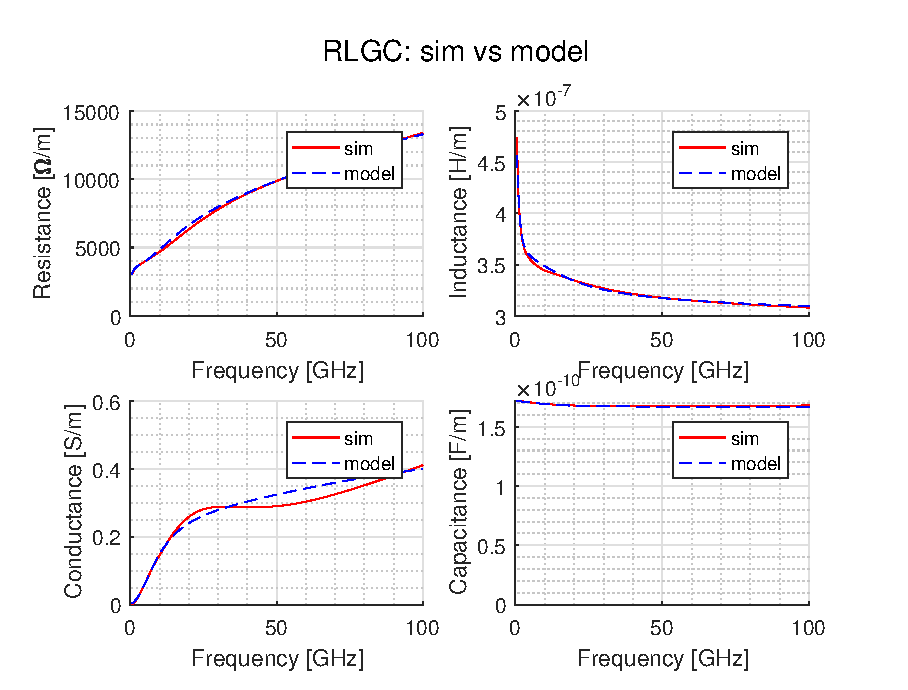
\includegraphics[width=7cm]{mymodel_25um.eps}}
 \hspace{0.1cm}
 %\qquad
  \subfloat[200um为标准选择模型级联个数]{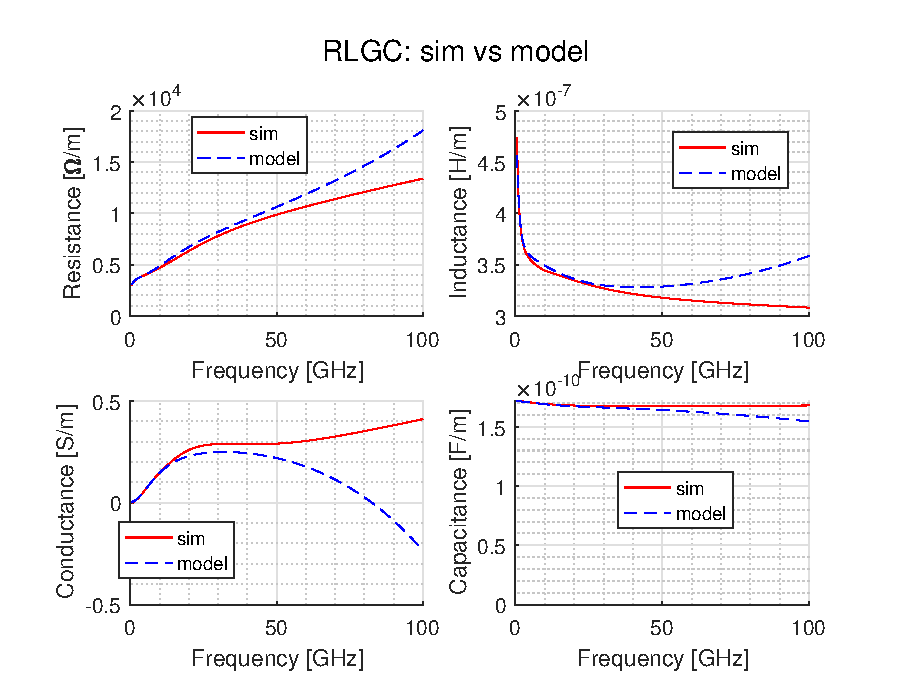
\includegraphics[width=7cm]{mymodel_200um.eps}}
  \vspace{0.5cm}
  \centering
   \caption{CPW :L$\times$S$\times$w=200um$\times$4um$\times$4um模型拟合结果和仿真结果对比} \label{fig:cmp_len}
\end{figure}

\section{方案对比-以CPW为例}
\subsection{THU方案和IBM方案对比}
IBM方案和THU方案采用类似结构,串联部分提参方法基本一致,IBM对模型并联部分进行了简化处理且不考虑G。均采用3段子电路形式级联,THU方案对200um长CPW进行拟合,模型拟合结果和仿真结果如图\ref{fig:thu_200};
IBM方案对100um长singleCPW模型进行拟合,模型拟合结果和仿真结果如图\ref{fig:ibm_100}。
\begin{figure}
  \centering
  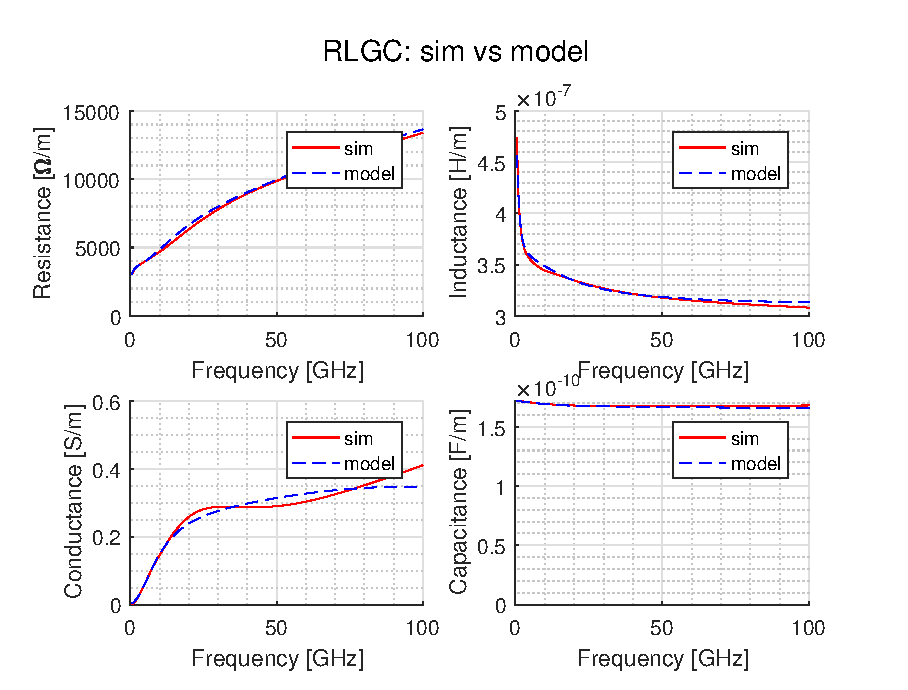
\includegraphics[width=12cm]{mymodel_70um.eps}
  \caption{THU方案模型拟合结果和仿真结果对比\ CPW :L$\times$S$\times$W=200um$\times$4um$\times$4um}\label{fig:thu_200}
\end{figure}

\begin{figure}
  \centering
  \includegraphics[width=14 cm]{IBM_sim.jpg}
  \caption{IBM方案模型拟合结果和仿真结果对比\ CPW :L$\times$W=100um$\times$5um}\label{fig:ibm_100}
\end{figure}

\subsection{THU方案和TSMC方案对比}
TSMC采用3个基本的$\pi$型单元级联,对于单个$\pi$型电路,其整体电阻和电感可计算得到如下:
\begin{gather}
  R(\omega)=\frac{R_1R_2}{R_1+R_2}\frac{1+(\frac{\omega}{\omega_1})^2}{1+(\frac{\omega}{\omega_2})^2} \label{equ:_pi_R}\\
  L_{(\omega)}=L_1+(\frac{R_1}{R_1+R_2})^2 \frac{L_2}{1+(\frac{\omega}{\omega_2})^2}
\end{gather}
其中$\omega_2=(R_1+R_1)/L_2$,$\omega_1=\omega_2\sqrt{R_2/(R_1+R_2)}$,从式\ref{equ:_pi_R}中,我们可以看到:
\begin{enumerate}[itemsep=1pt, topsep=12pt, partopsep=0pt,label={(\arabic*)}] %设置间距
  \item 当$\omega\ll\omega_1$时,R为常数
  \item 当$\omega_1 < \omega < \omega_2$时,R是递增的
  \item 当$\omega \gg \omega_2$时,R为常数
\end{enumerate}
R的这些特性和实际情况(见图\ref{fig:thu_200})不一样,实际情况下,在100GHz内电阻是随频率递增的,没有常数区域。
$\pi$型电路这一特性使得其参数提取变得困难,需要人工优化。更详细的分析见文件\cite{brinkhoff2008scalable}。
\par
THU方案中,基本电路模型的R和实际情况一致,参数提取方法成熟简单,容易实现较好的拟合结果。

\section{讨论}
\noindent
{\heiti 多个基本单元电路级联的必要性}\vspace{0.2 cm}
\par
从前面的分析可以看出,对于高频下的模型使用多个基本单元电路级联能实现对模型更好的拟合,拟合精度更高。\\

\noindent
{\heiti 回答邮件中的问题--根据模型长度变化模型电路架构}\vspace{0.2 cm}
\par
我后来也查了一些资料,使用spice语言好像是无法实现的,要实现这个功能需要一些其它的PDK实现的非常规操作,
如修改cadence保存并检查的按钮功能(cadence提供了编程接口),用户保存检查电路调用脚本重新生成模型定义文件,不过这并不是可取的办法。
\par
就目前来说,要想实现较好的等效电路模型,采用一个固定的多段图\ref{fig:my_model}级联的等效电路(保证最长尺寸的精度要求,对其它尺寸相当于是冗余的)模型是最为可行的,
具体采用多少段拼接还需要后续根据实际scalabe公式拟合误差以及精度要求等修正,验证。
\par
经过测试,就采用100段图\ref{fig:my_model}模型级联和单独使用1段图\ref{fig:my_model}模型,使用matlab进行仿真计算得到其S参数,耗时情况如下表:
\begin{table}[hbt]
\centering
\caption{用matlab进行仿真计算得到其S参数耗时分析}
\label{table:time}
\begin{tabular}{|c|c|}
\hline
级联数 & 仿真耗时(s)  \\ \hline
1   & 0.006511 \\ \hline
100 & 0.008107 \\ \hline
\end{tabular}
\end{table}
虽然没有用cadence等软件进行测试,但matlab测试结果来看,采用
多段级联的方式给电路仿真带来的时间开销几乎可以忽略不计,采用100段模型级联计算中占用的内存也是非常少的。
\par
对于采用多段模型级联的方式,其模型定义文件中等效电路网表定义语句会比较多,但是模型定义文件只需要编写一次,而且其等效电路网表完全可以用cadence等软件直接生成、无需自己编写,由于其只是简单的循环也较容易使用matlab等编程工具实现电路网表生成。


\vspace{0.2 cm}
\noindent
{\heiti TSMC模型存在的问题}\vspace{0.2 cm}
\par
TSMC模型的提参数方法并没有公开的较好的方法,一般需要较多的手工或是算法调优,要实现其能够应用到100GHz下,应该也需要使用多段级联的结构。
\par
可能通过调节参数以及采用更多段级联的方式可以使TSMC的模型能够应用到100GHz下,除去提取参数复杂的这一缺点,
目前没找到任何支撑的材料可以证明其采用TSMC模型能够比THU模型用更少的级联段数实现相同的拟合精度。


\vspace{0.2 cm}
\noindent
{\heiti 采用固定的较少的THU模型级联通过优化参数的方式来实现对模型整体(而不是目前单位长度)参数的拟合}\vspace{0.2 cm}
\par
个人觉得这是可以做到的,但是那样的话需要抛弃现有的提参方法,因为此模型并不是基于物理的模型,有如下两个明显的缺点:
\begin{enumerate}[itemsep=1pt, topsep=12pt, partopsep=0pt,label={(\arabic*)}] %设置间距
  \item 由于元件个数较多,而且THU模型本身的物理意义并不太明确,元件取值无太多的限制,多自由变量下的提参将变得困难
  \item 那样建模提取出来的参数与元件长度L会是复杂的函数关系,由于多了一个变量,这对建立scalable模型增加了一个维度,难度将增加很多,需要用来提取参数的模型也要若干倍的增加
\end{enumerate}
因此这种方式,会比目前更加复杂,工程耗时也将增多非常多。
\vspace{0.2 cm}


\vspace{0.2 cm}
\noindent
{\heiti 其它}\vspace{0.2 cm}
\par
由于我个人工程经验不足,从事着方面的研究学习的时间也非常短,有一些地方可能不太了解,还希望你们能指出:
\begin{itemize}
  \item THU模型在实际应用中会存在的问题?
  \item TSMC模型在实际应用中的优势?
\end{itemize}
\vspace{0.2 cm}
\bibliography{myRef}
\end{document} 